\documentclass[a4paper]{article}
\usepackage[english]{babel}
\usepackage{xltxtra}
\usepackage{hyperref}
\usepackage{listings}
\usepackage{graphicx}
%\usepackage[a4paper]{geometry}
\begin{document}
\title{\vspace{-1.0cm}Artificial Intelligence II -- Homework 3 \\ \textbf{8 queens puzzle}}
\author{Jonáš Petrovský\\
        Faculty of Business and Economics,\\
		Mendel University in Brno,\\
		Czech Republic \\
		\texttt{jond@post.cz}}
\date{\today}
\maketitle

\section{Introduction}
The goal of the work is to implement a solution to the ''8 queens puzzle'' using the "MIN-conflict" heuristic. There are 8 queens on a chess board. The goal is to rearrange the queens so that no two queens threaten each other.

\section{Solution design}
There are 4,426,165,368 possible arrangements of eight queens on an 8×8 board, but only 92 solutions (Wikipedia, 2015). We could use brute-force, but there exists a smarter way. We apply a rule that in one column can only be one queen. Then we use the MIN-conflict heuristic to select the best following state.

\section{Implementation}
The program was implemented in Python. A state is saved as a 2D array representing a chess board, where 1 means there is a queen on the square and 0 that there is no queen. Example for lecture state 1:
\begin{lstlisting}[language=python]
state = [
            [0,0,0,0,1,0,0,0],
            [1,0,0,0,0,0,0,0],
            [0,0,0,0,0,1,0,0],
            [0,0,0,1,0,0,0,0],
            [0,1,0,0,0,0,0,0],
            [0,0,0,0,0,0,1,0],
            [0,0,1,0,0,0,0,0],
            [0,0,0,0,0,0,0,1],
]
\end{lstlisting}
All visited states are saved in ''solution\_path'' list (in order). There is a main class \textbf{ChessQueenWorld} with following public methods: 
\begin{itemize}
\item \verb|solve_given_board(start_state)|
\item \verb|solve_random_board()|
\item \verb|solve_sample_board(number)|
\item \verb|bulk_solve(number_of_boards)|
\end{itemize}

The main method \verb|solve_given_board()| accepts a start state and tries to find a solution using the heuristic.
\begin{enumerate}
\item Reset a solution path.
\item Insert a start state into the solution path.
\item While conflicts count > 0 OR iterations count <= 500:
	\begin{enumerate}
	\item Choose a new queen position with min. number of conflicts.
	\item Check if the new state is already in solution path.
	\item If yes, re-run the method.
	\item If not, add it to the solution.
	\end{enumerate}
\end{enumerate}
If there are no conflicts, a message of success and number of performed moves are displayed.

Class \textbf{QueenHeuristics} implements the calculation of ''MIN-conflict'' heuristic. For every column, we try to place a queen  on different squares and count the number of conflicts on every position. Than the position with the lowest number is chosen. However, if the count is higher than count on the queen's original position, we choose nothing.

Class \textbf{StatesCreator} contains sample states and \verb|generate_random_start_state()| method.

There is a simple test class in folder /tests, which can be used to check (for sample states), whether heuristic method returns the correct number of conflicts for given state. The class can be used in \verb|test-3-check.py| file.

The program can be run by typing the following command into the operating system's terminal (Python 2.7 has to be installed on the system): \\ 
\verb|python run-3.py| \\
What the program should do must be stated in the run-3.py source code (the script has no parameters).

\section{Results}
All resulting text files are placed in /output folder. The first matrix is the start state, then the performed steps and the final state are displayed.

\subsection{Lecture start states}
\textbf{Board 1} (1 conflict): Solved in 2 steps. More in lecture\_1.txt. \\
\textbf{Board 2} (28 conflicts): Solved in 10 steps. More in lecture\_2.txt.

\subsection{Generated start states}
The method \verb|generate_random_start_state()| can be used to produce some of the 16,777,216 possible queens combinations  (one queen in every column). ''Efficiency'' means average number of steps (queen moves) for solution. ''Success rate'' shows how many percent of the generated start states has the algorithm been able to solve.  

\renewcommand{\arraystretch}{1.5}
\begin{table}[h!]
\centering
\caption{Total results generated start states}
\label{table:totalres}
\begin{tabular}{ | l | c| c|c|}
\hline
N. of boards & 100 & 1,000 & 10,000 \\ 
\hline
Success rate [\%] & 96 & 95.2 & 94.37 \\
Efficiency [steps] & 18.34 & 17.6 & 17.49 \\
\hline
\end{tabular}
\end{table}

From Table \ref{table:totalres} can be seen that the algorithm managed to solve the overwhelming majority of generated boards (95 \%) in 17 steps on average. 

Subsequently, the number of conflicts in the start states and its impact on success rate and efficiency is examined. We take values from simulation of 10,000 boards to present the most accurate conclusions.

\begin{figure}[ht!]
\centering
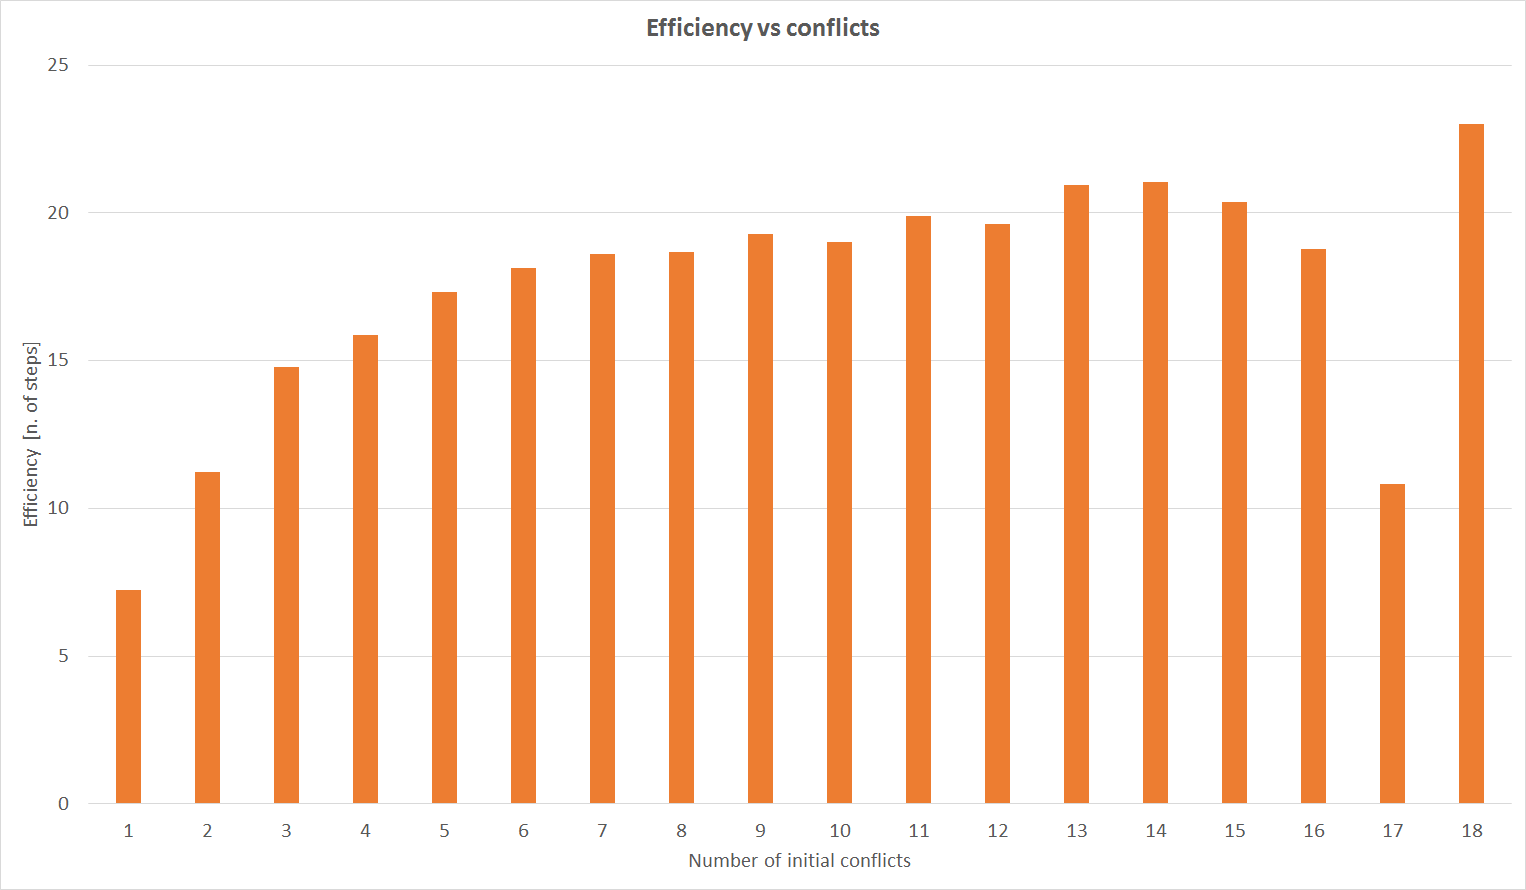
\includegraphics[width=\textwidth]{eff-chart.png}
\caption{Relation between number of initial conflicts and efficiency} 
\label{fig:eff}
\end{figure}

As can be seen in Figure \ref{fig:eff}, there is an obvious correlation between number of initial conflicts and efficiency -- the more initial conflicts, the more steps need to be performed (on average).  Of course, there are some irregularities, but on the whole, the conclusion is correct. 

The success rate was 100 \%, except for 1, 17 and 18 initial conflicts, where the rate was 10.81, 5.83 and 50 \%, respectively. The overwhelming majority (94~\%) of generated states contained 3--14 conflicts (categories with more than 100 states). The aforementioned success rate might be the result of too low number of tested examples, but also a high complexity of the given start states. For a detailed examination a larger number of generated states would be needed.


\section{References}

Eight queens puzzle. \textit{Wikipedia: the free encyclopedia} [online]. San Francisco (CA): Wikimedia Foundation, last updated 3. 12. 2015 [accessed 2015-12-05]. Available at: https://en.wikipedia.org/wiki/Eight\_queens\_puzzle


\end{document}  %End of document.